\subsection{UkuTabs}

UkuTabs\cite{ukuleletabs_home} es una aplicación web diseñada principalmente para el ukelele, aunque también ofrece soporte para otros instrumentos como la guitarra y el mandolín. Entre las páginas que componen la aplicacion destacamos las relacionadas con canciones, herramientas y las informativas.

En primer lugar, con respecto a las \textbf{páginas relacionadas con canciones}, podemos encontrar:

\begin{itemize}
    \item \textbf{Biblioteca de canciones} (véase Figura~\ref{fig:ukutabs_home}), con la posibilidad de realizar búsquedas avanzadas por género, artista, popularidad, dificultad, listas (navideñas, infántiles\ldots) o tipo (acordes, tablaturas o ambas).
    \item \textbf{Canciones} (véase Figura~\ref{fig:ukutabs_somewhereovertherainbow}), que contienen la letra, acordes y utilidades~(véase Tabla \ref{tab:ukutabs_utilidades_canciones}) para la práctica de las mismas.
    \item \textbf{Solicitudes} de nuevas canciones.
\end{itemize}

En segundo lugar, en cuanto a las \textbf{páginas informativas y herramientas}, podemos encontrar:
\begin{itemize}
    \item \textbf{Guías} (véase Figura~\ref{fig:ukutabs_guias}), con un listado de lecciones que abarcan todos los aspectos necesarios para introducirse al ukelele.
    \item \textbf{Diccionario de acordes} (véase Figura~\ref{fig:ukutabs_acordes}), que permite realizar búsquedas de acordes con la posibilidad de ser visualizada a través de un diagrama o en una simulación del mástil del instrumento.
    \item \textbf{Calculadora de escalas o notas}, que al introducir una nota muestra los resultados en una simulación del mástil del instrumento
    \item \textbf{Afinador de instrumento interactivo}, haciendo uso del micrófono integrado en el dispositivo.
\end{itemize}

\begin{figure}[H]
    \centering

    % Primera fila
    \begin{subfigure}[t]{0.48\textwidth}
        \centering
        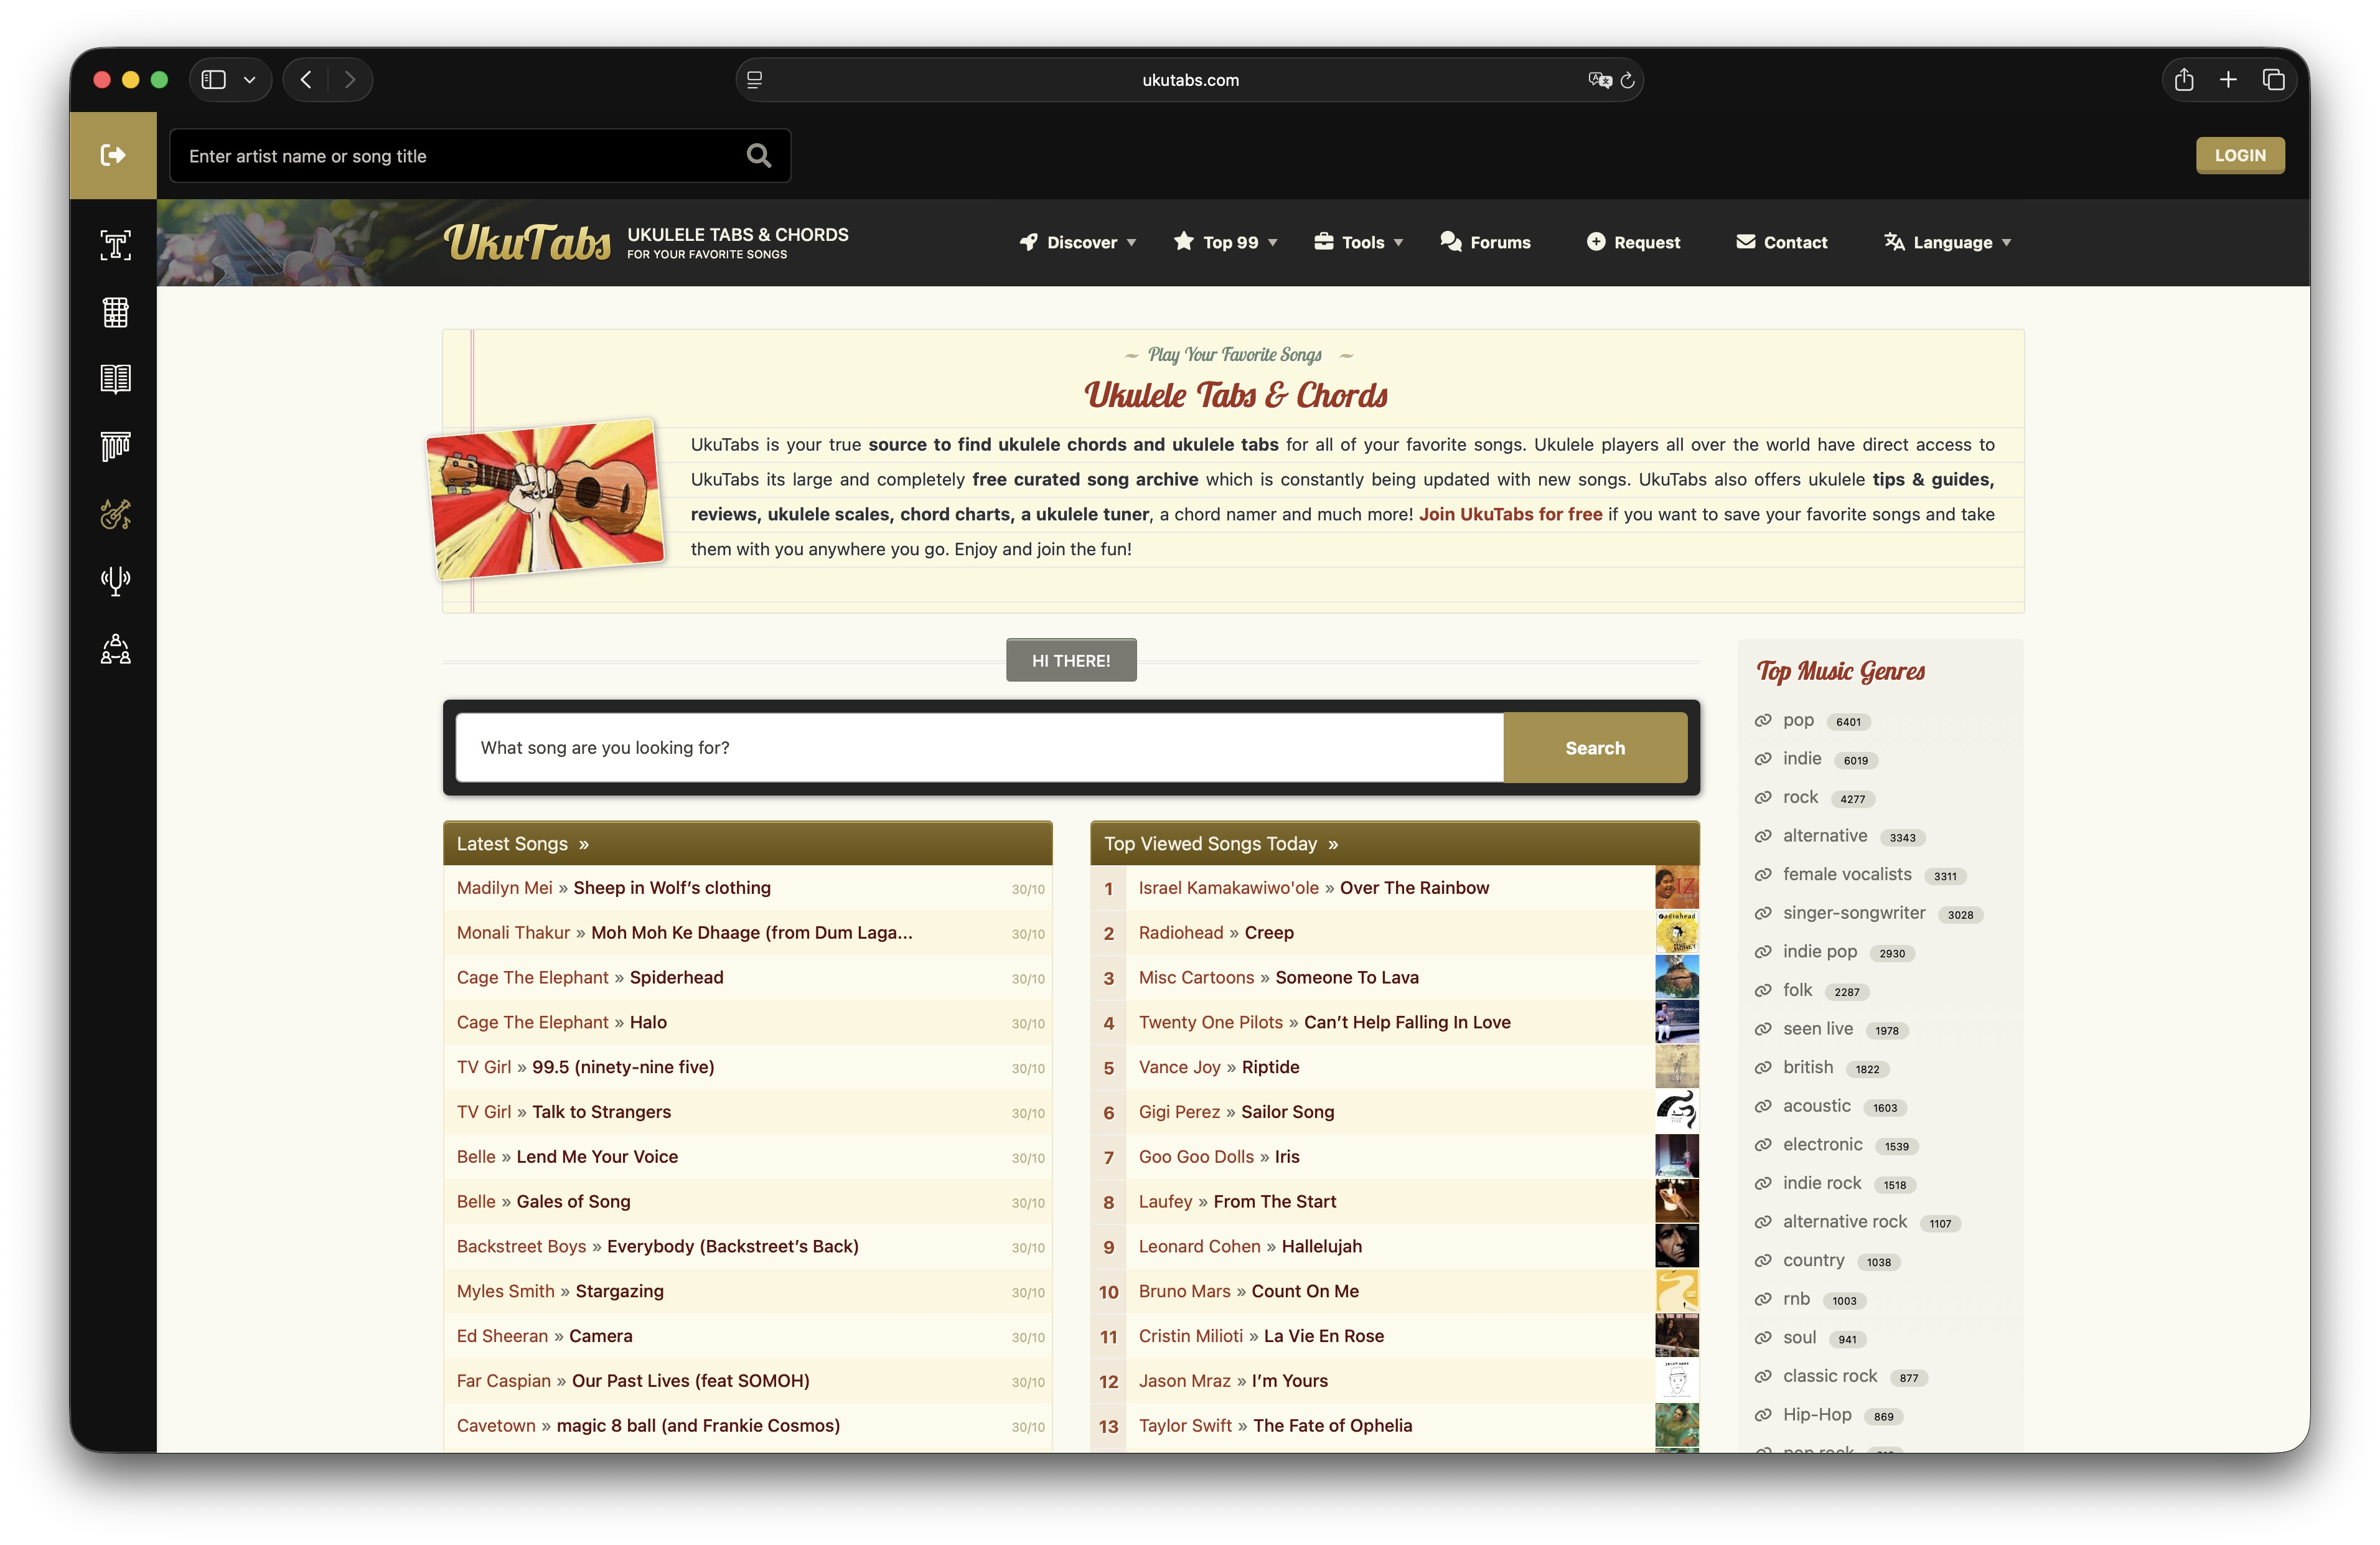
\includegraphics[width=\textwidth]{Ilustraciones/estado/ukutabs.jpeg}
        \caption{Página principal de UkuTabs~\cite{ukutabs_home}}
        \label{fig:ukutabs_home}
    \end{subfigure}
    \hfill
    \begin{subfigure}[t]{0.48\textwidth}
        \centering
        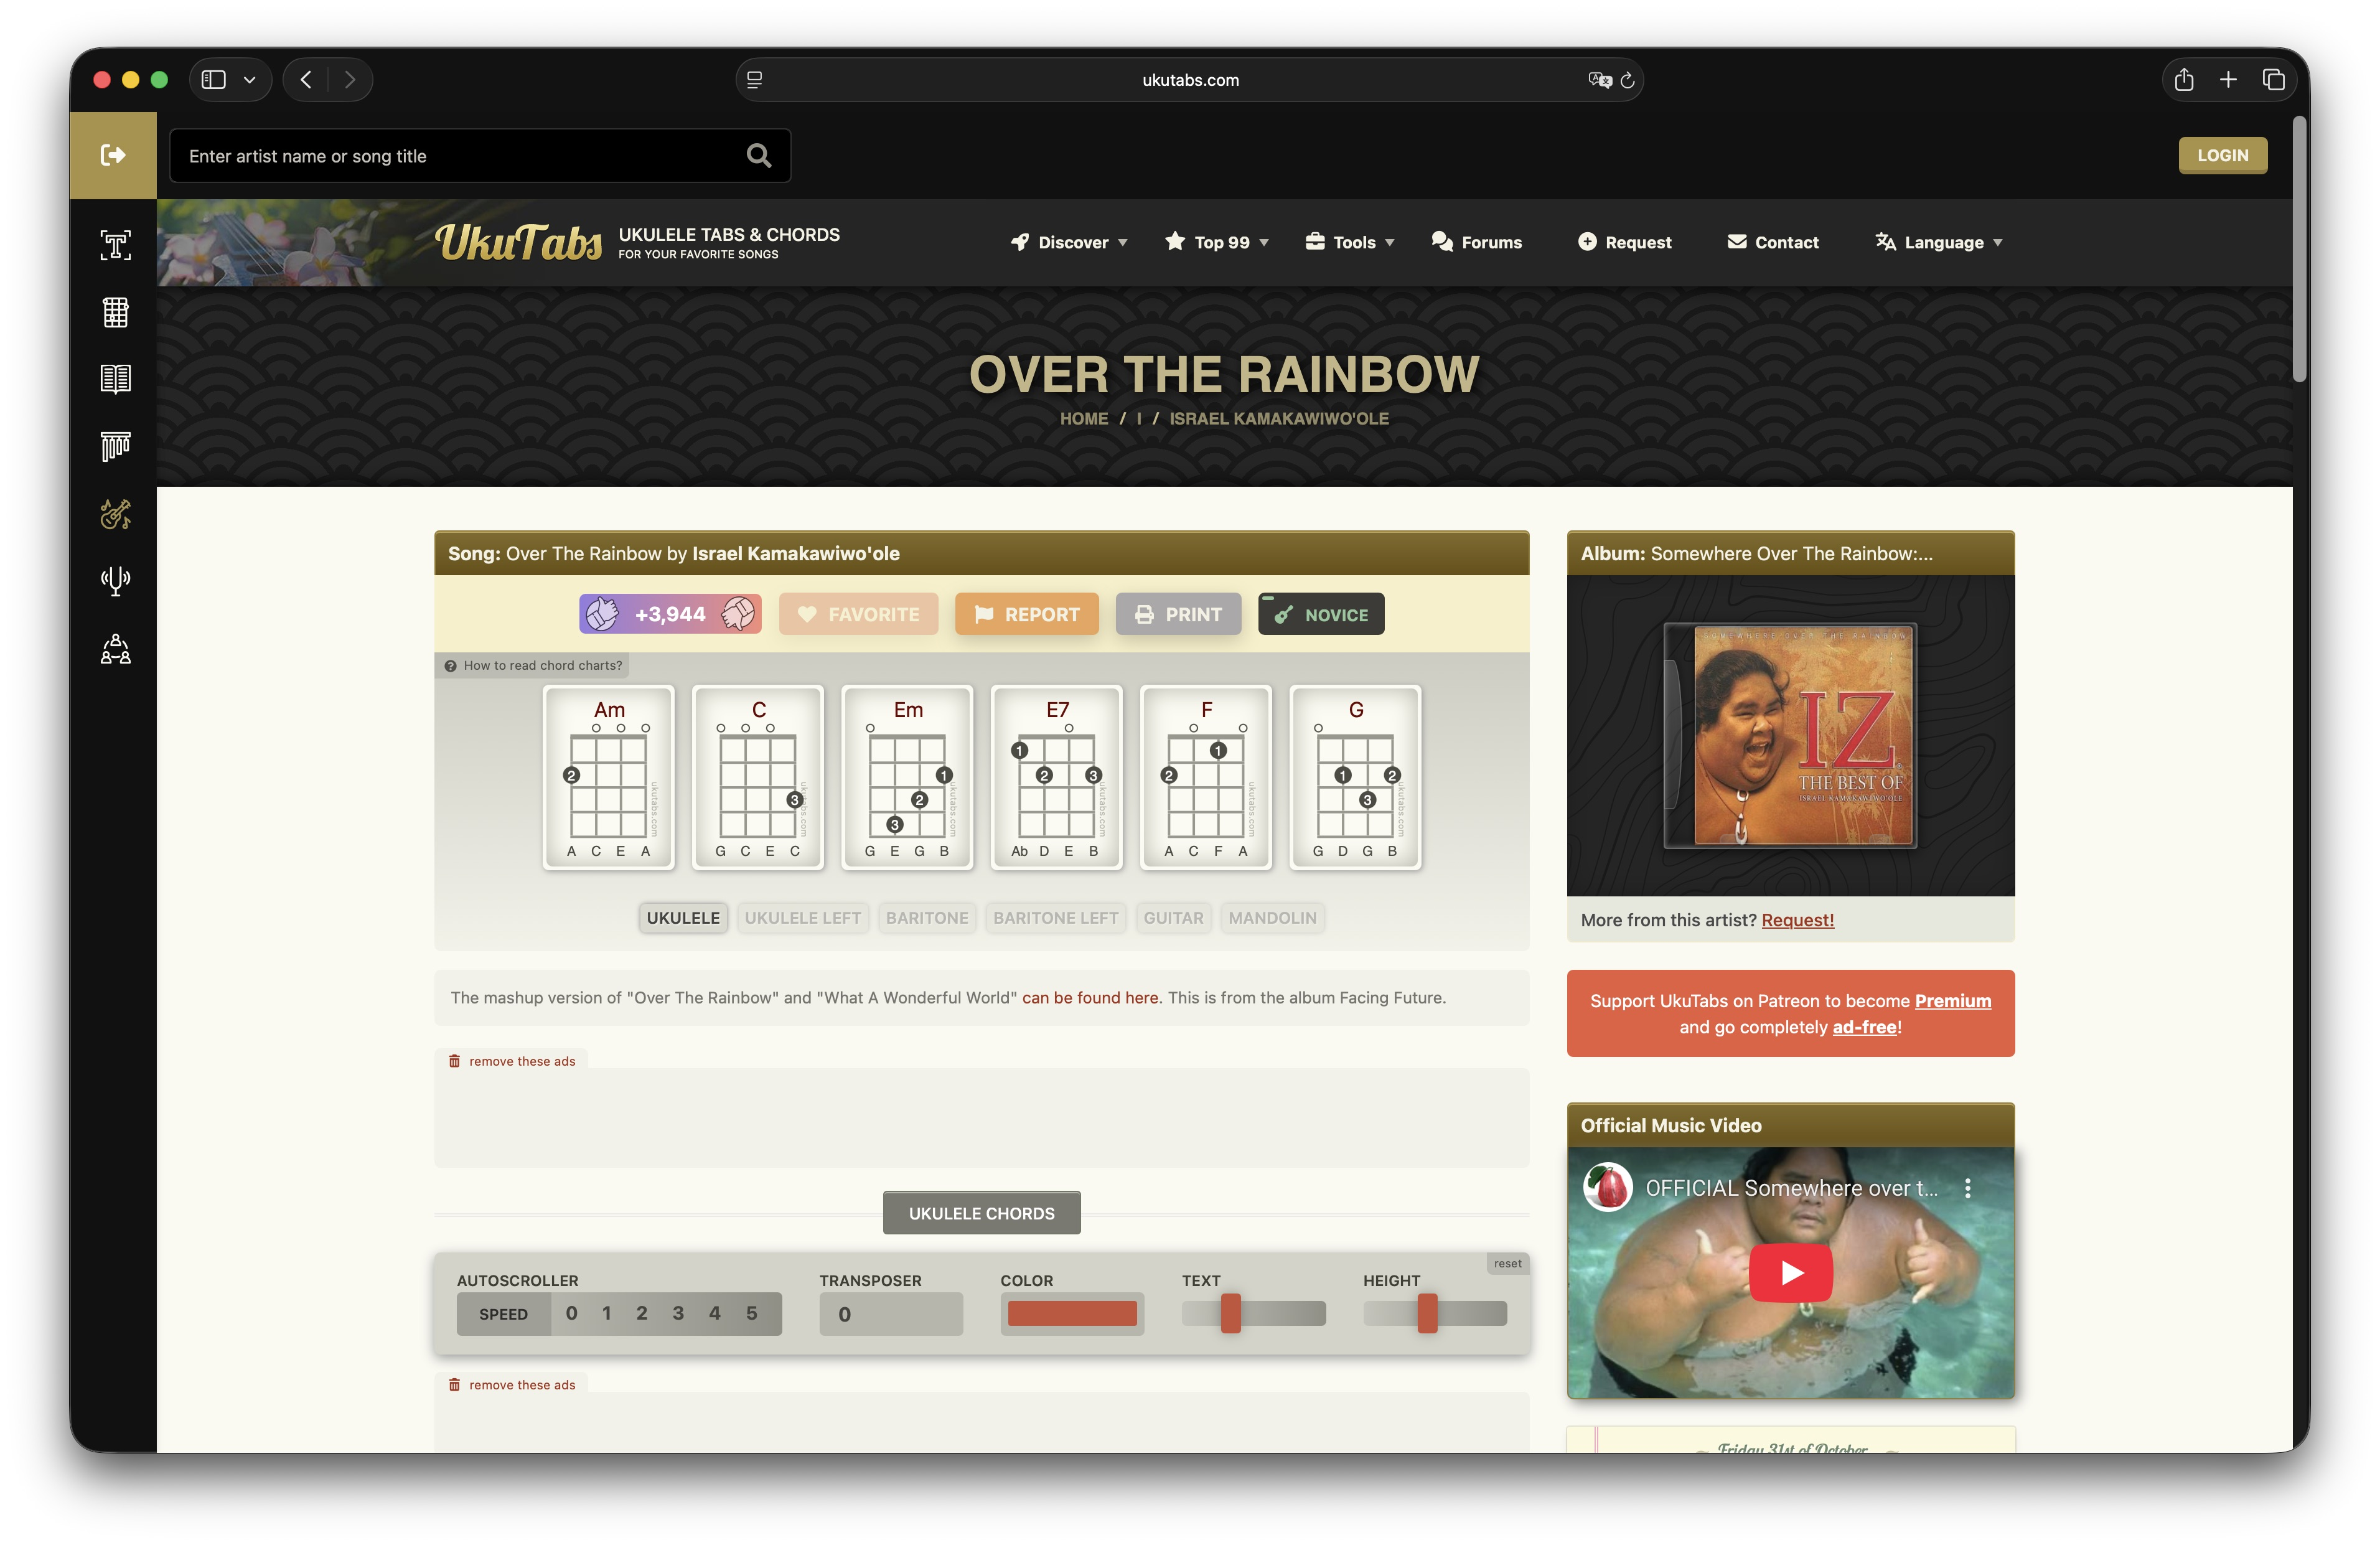
\includegraphics[width=\textwidth]{Ilustraciones/estado/ukutabs_somewhereovertherainbow.jpeg}
        \caption{Acordes y letra de \emph{Somewhere over the rainbow}~\cite{ukutabs_somewhereovertherainbow} para ukelele en UkuTabs}
        \label{fig:ukutabs_somewhereovertherainbow}
    \end{subfigure}

    \vspace{1em} % Espacio vertical entre filas

    % Segunda fila
    \begin{subfigure}[t]{0.48\textwidth}
        \centering
        \includegraphics[width=\textwidth]{Ilustraciones/estado/ukutabs_guías.jpeg}
        \caption{Página de guías de UkuTabs~\cite{ukutabs_guias}}
        \label{fig:ukutabs_guias}
    \end{subfigure}
    \hfill
    \begin{subfigure}[t]{0.48\textwidth}
        \centering
        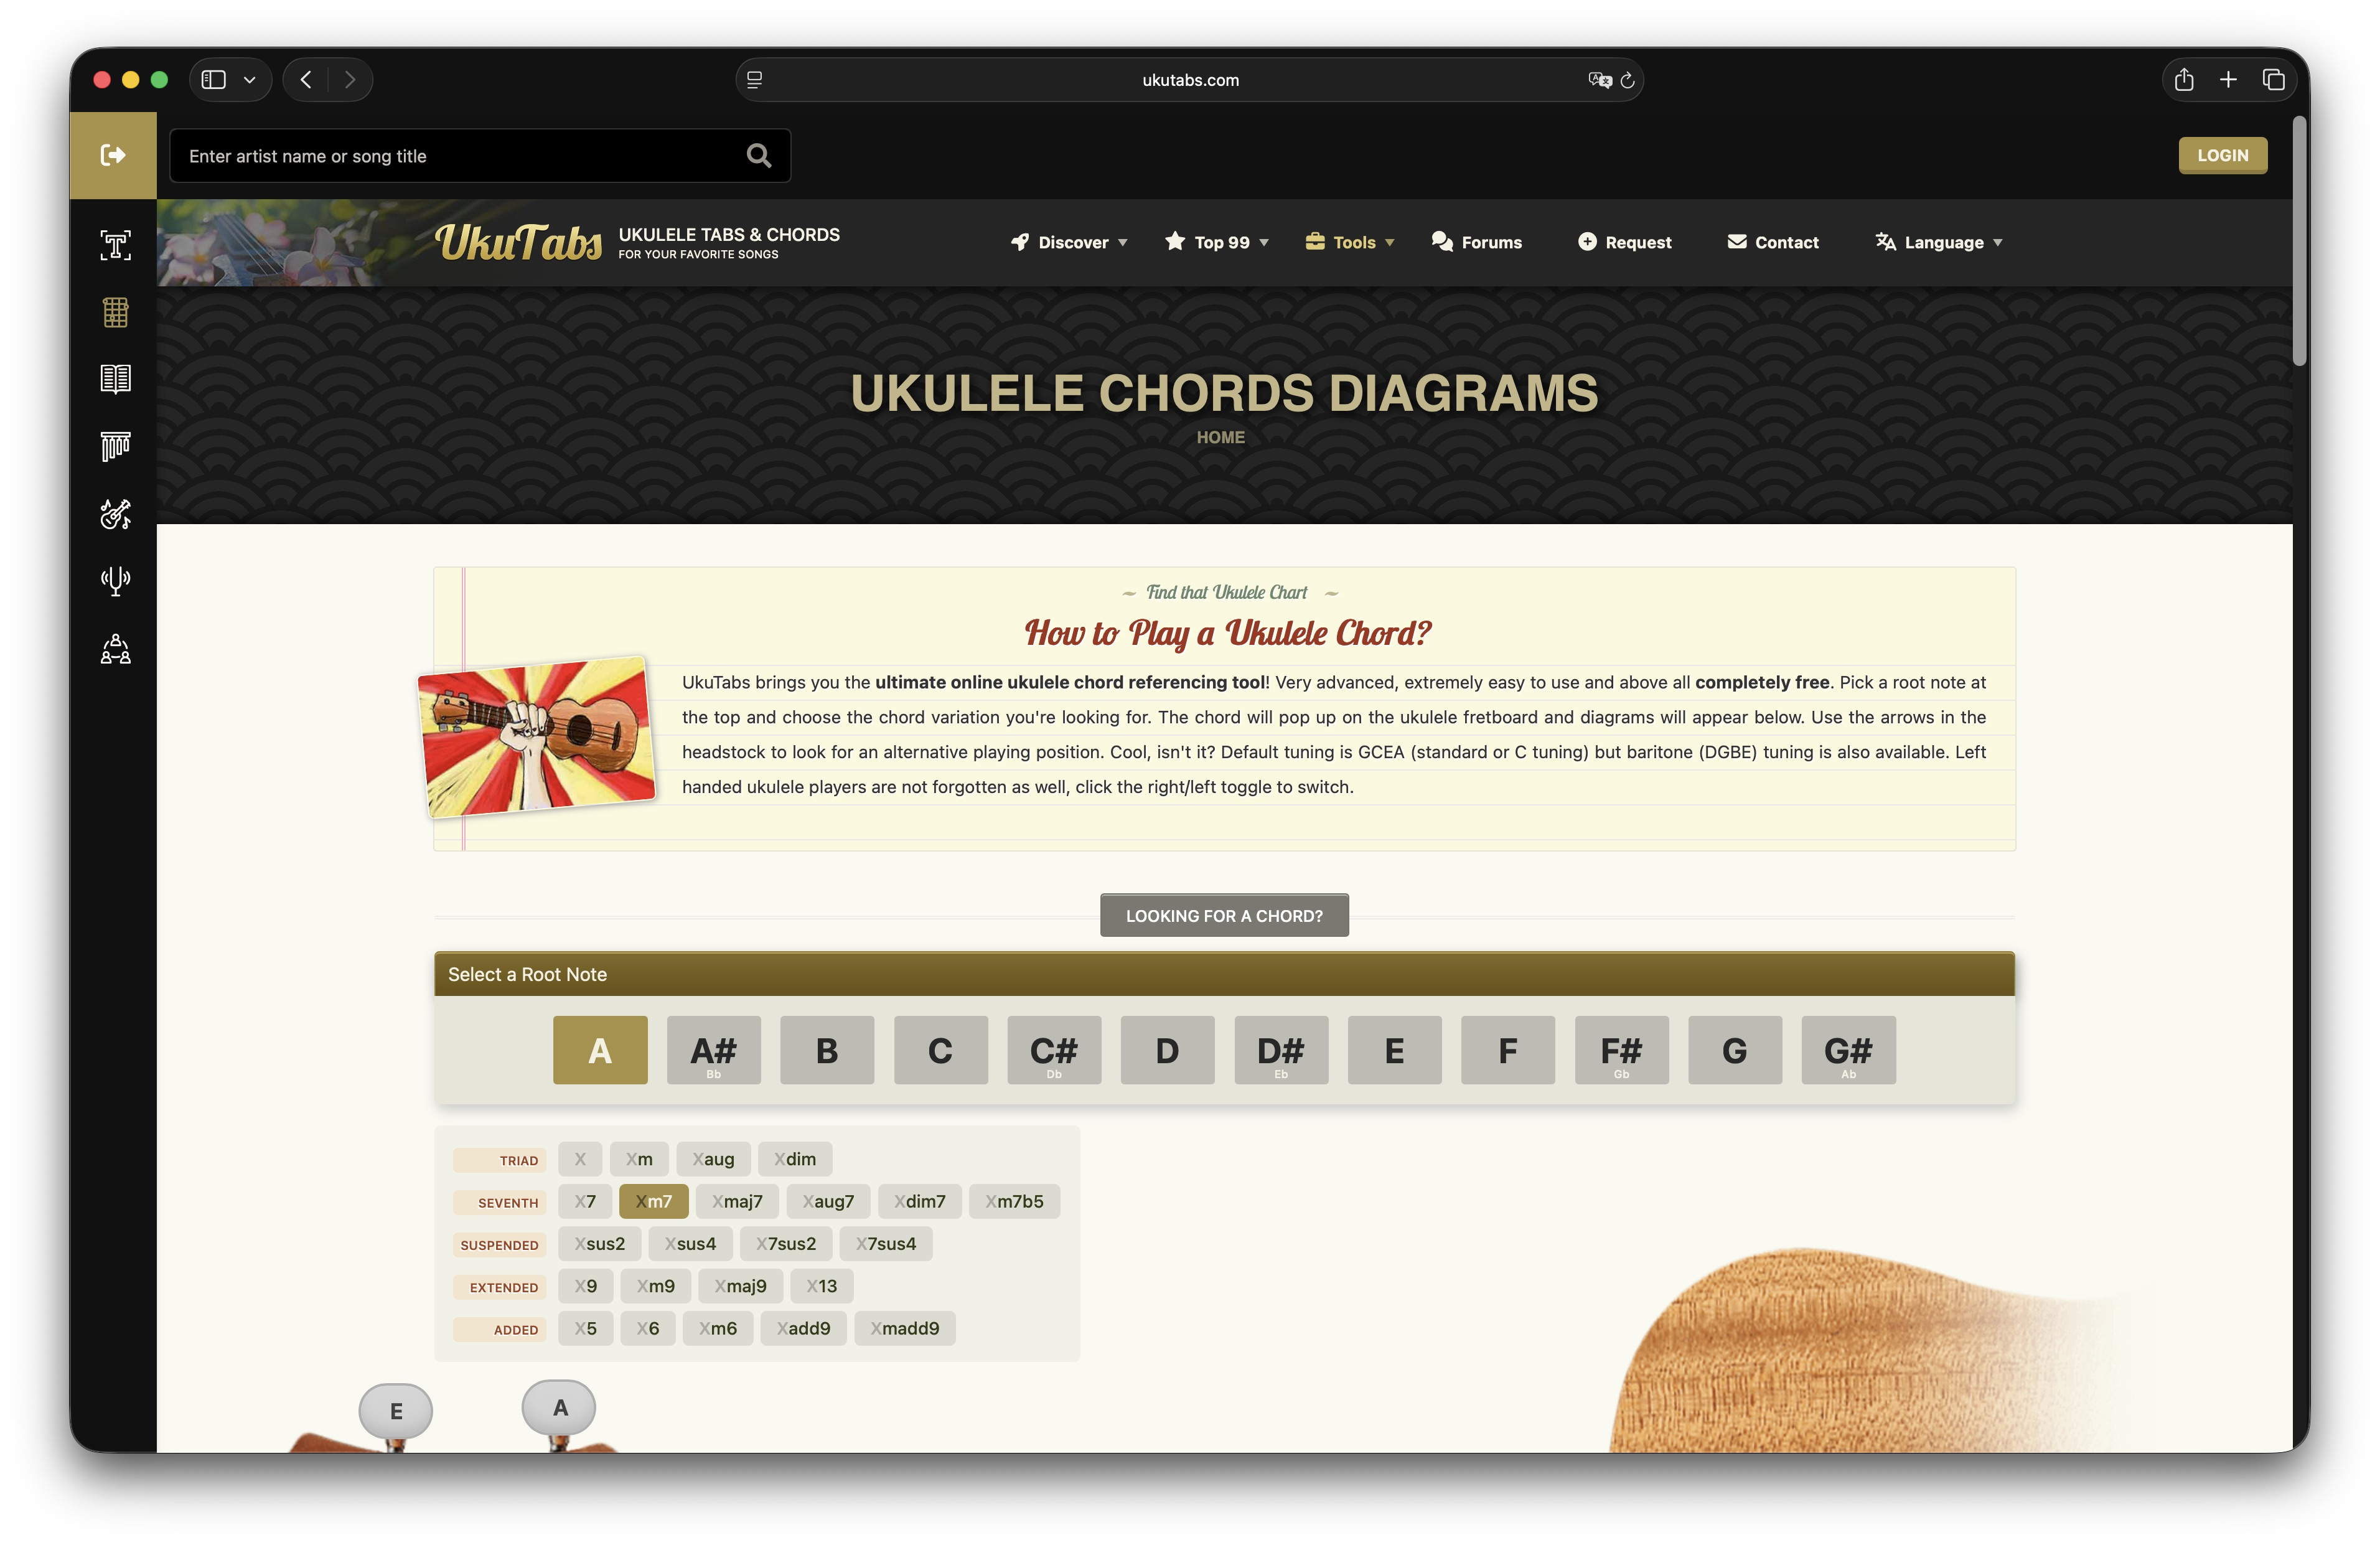
\includegraphics[width=\textwidth]{Ilustraciones/estado/ukutabs_acordes.jpeg}
        \caption{Página de acordes de UkuTabs~\cite{ukutabs_acordes}}
        \label{fig:ukutabs_acordes}
    \end{subfigure}

    \caption{Páginas de UkuTabs.}
    \label{fig:ukutabs_canciones}
\end{figure}

En conclusión, UkuTabs es una aplicación web muy cuidada, tanto en el nivel funcional como en el visual. Nos encontramos ante un producto que ofrece una experiencia de usuario completa y eficaz, con un gran número de herramientas interactivas y un sistema de verificación de contenido mediante administradores que garantiza la calidad de sus contenidos. Además, la aplicación se monetiza a través de anuncios, lo que permite el acceso gratuito a sus usuarios, poniendo a su disposición la mayoría de sus funcionalidades sin necesidad de registro (véase Tabla~\ref{tab:ukutabs_funcionalidades_usuario}).

\begin{table}[H]
    \scriptsize
    \begin{minipage}[t]{0.4\textwidth}
        \centering
        \caption{Utilidades presentes en publicaciones de UkuTabs}\label{tab:ukutabs_utilidades_canciones}
        \begin{tabular}{l c}
            \hline
            \textbf{Utilidad} & \textbf{Existe} \\
            \hline
            Transportador & \ding{51} \\
            Lista de acordes & \ding{51} \\
            Autodesplazamiento & \ding{51} \\
            Impresión/Descarga & \ding{51} \\
            Cambio de notación &  \\
            Cambio de instrumento & \ding{51} \\
            Guardar canción & \ding{51} \\
            Guía de rasgueos & \\
            \hline
        \end{tabular}
    \end{minipage}
    \hfill
    \begin{minipage}[t]{0.56\textwidth}
        \centering
        \caption{Funcionalidades disponibles según el rol del usuario de UkuTabs}\label{tab:ukutabs_funcionalidades_usuario}
        \begin{tabular}{l c c }
            \hline
            \multirow{2}{*}{\textbf{Funcionalidad}} & \multicolumn{2}{c}{\textbf{Rol Uusario}} \\
            & Visitante & Registrado \\
            \hline
            % --- Ejemplo de fila vacía (borra o completa) ---
            Biblioteca de canciones & \ding{51} & \ding{51} \\
            Creación y edición de publicaciones &  & \ding{51}  \\
            Utilidades de publicaciones & \ding{51} & \ding{51} \\
            Puntuar publicaciónes &  & \ding{51}  \\
            Comentar publicaciones &  & \ding{51}  \\
            Solicitar nuevas canciones & \ding{51}  & \ding{51}  \\
            Cursos y guías & \ding{51} & \ding{51} \\
            Afinador & \ding{51} & \ding{51}  \\
            Calculadora de escalas y notas & \ding{51} & \ding{51}  \\
            Diccionario de acordes & \ding{51} & \ding{51}  \\
            % ------------------------------------------------
            \hline
        \end{tabular}
    \end{minipage}
    
\end{table}